\documentclass{article}

\usepackage{amssymb,amsmath,multicol,enumerate,amsthm,graphicx}

\usepackage{enumerate}
\usepackage{color}
\usepackage{xcolor}
\usepackage{listings}
\usepackage{mathtools}
\usepackage{graphicx}
\graphicspath{ {./} }
\usepackage{pgfplots}
\usepackage{./bluespec}
\usepackage{svg}

\usepackage{graphicx} % Required for inserting images
\usepackage[margin=1in]{geometry}   % Marges
\usepackage{latexsym}
\usepackage{amssymb}
\usepackage{amsmath}
\usepackage{amsfonts}
\usepackage{verbatim}
% \usepackage{listings}
\DeclareSymbolFont{largesymbols}{OMX}{cmex}{m}{n} % However for large sigmas we want the Computer Modern symbol
\renewcommand{\ttdefault}{cmtt}
\usepackage{array}
\usepackage{multirow}
\usepackage{color}
\usepackage{xspace} % xspace takes care of the \@ after a capitalized word before a period.
\usepackage{multicol}
\usepackage{graphicx}
\usepackage{fancyhdr}

\setlength{\oddsidemargin}{0pt}
\setlength{\evensidemargin}{0pt}
\setlength{\textwidth}{6.5in}
% \setlength{\topmargin}{-1in}
% \setlength{\bottommargin}{-1in}
% \setlength{\textheight}{8.5in}
% \usepackage[margin=1in]{geometry}
\setlength{\parskip}{1pc}
\setlength{\parindent}{0pt}

\lstdefinelanguage{RSVAssembler}
{
  alsoletter={.}, % allow dots in keywords
  alsodigit={0x}, % hex numbers are numbers too!
  morekeywords=[1]{ % instructions
    lb, lh, lw, lbu, lhu,
    sb, sh, sw,
    sll, slli, srl, srli, sra, srai,
    add, addi, sub, lui, auipc,
    xor, xori, or, ori, and, andi,
    slt, slti, sltu, sltiu,
    beq, bne, blt, bge, bltu, bgeu,
    j, jr, jal, jalr, ret,
    scall, break, nop
  },
  morekeywords=[2]{ % sections of our code and other directives
    .align, .ascii, .asciiz, .byte, .data, .double, .extern,
    .float, .globl, .half, .kdata, .ktext, .set, .space, .text, .word
  },
  morekeywords=[3]{ % registers
    zero, ra, sp, gp, tp, s0, fp,
    t0, t1, t2, t3, t4, t5, t6,
    s1, s2, s3, s4, s5, s6, s7, s8, s9, s10, s11,
    a0, a1, a2, a3, a4, a5, a6, a7,
    ft0, ft1, ft2, ft3, ft4, ft5, ft6, ft7,
    fs0, fs1, fs2, fs3, fs4, fs5, fs6, fs7, fs8, fs9, fs10, fs11,
    fa0, fa1, fa2, fa3, fa4, fa5, fa6, fa7
  },
  morecomment=[l]{;},   % mark ; as line comment start
  morecomment=[l]{\#},  % as well as # (even though it is unconventional)
  morestring=[b]",      % mark " as string start/end
  morestring=[b]'       % also mark ' as string start/end
}


\lstset{language=[Bluespec]Verilog,keywordstyle={\bfseries \color{blue}}}

\definecolor{mygreen}{rgb}{0,0.6,0}
\definecolor{mygray}{rgb}{0.5,0.5,0.5}
\definecolor{mymauve}{rgb}{0.58,0,0.82}
\definecolor{codegreen}{rgb}{0,0.6,0}
\definecolor{codegray}{rgb}{0.5,0.5,0.5}
\definecolor{codepurple}{rgb}{0.58,0,0.82} 
\definecolor{backcolour}{rgb}{0.95,0.95,0.92}


\lstset{ %
  backgroundcolor=\color{white},   % choose the background color
  basicstyle=\footnotesize,        % size of fonts used for the code
  breaklines=true,                 % automatic line breaking only at whitespace
  captionpos=b,                    % sets the caption-position to bottom
  commentstyle=\color{mygreen},    % comment style
  escapeinside={\%*}{*)},          % if you want to add LaTeX within your code
  % morekeywords=[1]{arg,pos},
  keywordstyle=\color{blue},       % keyword style
  stringstyle=\color{mymauve},     % string literal style
  backgroundcolor=\color{backcolour},   
    commentstyle=\color{codegreen},
    keywordstyle=\color{magenta},
    numberstyle=\tiny\color{codegray},
    stringstyle=\color{codepurple},
    basicstyle=\ttfamily\footnotesize,
    breakatwhitespace=false,         
    breaklines=true,                 
    captionpos=b,                    
    keepspaces=true,                 
    numbers=left,                     
    numbersep=5pt,                  
    showspaces=false,                
    showstringspaces=false,
    % keywordstyle=\color{weborange},
    showtabs=false,                  
    tabsize=2
}



\title{6.175 Final Project Report}
\author{Lasya Balachandran, Sanjay Seshan\\lasyab@mit.edu, seshan@mit.edu}
\date{\today}

\begin{document}

% An approximately one-page description of your project idea is due on Friday 14th.
% Your report should describe the architecture techniques you will explore, design, and implement.
% Typically, most groups should probably first connect the process they wrote to a cache, and then
% upgrade the processor in two dimensions: to go superscalar, or SMT, or multicore, vectors or
% connecting an accelerator to the processor (the lecture about the last two will be given next week).
% 1
% You might also want to use an FPGA for your project, if you want to do so, you should say it in
% your proposal.
% For projects that would not be directly related to processors, you will need to be already very
% familiar with the domain and specific application you are trying to tackle and you should send us
% an email to fix a meeting with us next week to decide on reachable objectives.


\maketitle

\section{Introduction}

In this paper, we present our process and implementation of 6.175 design project. We chose to implement a working dual core processor with a functioning cache hierarchy and parent protocol processor. For the second part, we decided to run our code on an AWS FPGA.

\section{Cache and Processor}

In labs 4 and 5 we implemented a single core 32-bit RISC-V processor and a single level cache. The first step of our project was to create a single core processor with a L1 cache. However, to merge our code we had a few shortcomings that had to be addressed. 

\begin{enumerate}[(1)]
    \item The original cache only stores lines, but the processor stores words
    \item The processor has two types of data in DRAM -- instructions and data -- that was handled by a 2 port BRAM, but our cache has to use a single ported main memory
    \item Our \lstinline{mem.vmh} stored words, but we needed lines (16 words per line)
    \item Our cache interface was incompatible with the processor's request system
    \item The processor expects half words and byte storing
\end{enumerate}

To start our conversion to words, we made the system handle four offset bits, rather than returning or writing a whole line. Requests to and fro main memory remain lines.

We used the following definition of an address to index into the cache. 
\begin{lstlisting}
function CacheReqWorking extract_bits(CacheLineAddr addr, CacheReq e);
  let tag = addr[31:13];
  IndexAddr index = addr[12:6];
  let offset = addr[5:2];
  return CacheReqWorking{tag:tag,idx:index,offset:offset,memReq:e};
endfunction
\end{lstlisting}
Furthermore, we created two BRAMs. This allows us to use the byte enable feature on the data while storing tags and miss/hit/valid bits separately. 
\begin{lstlisting}
BRAM1Port#(IndexAddr, CacheReqLine) bram1 <- mkBRAM1Server(cfg);
BRAM1PortBE#(IndexAddr, Vector#(16, Word), 64) bram2 <- mkBRAM1ServerBE(cfg2);
\end{lstlisting}

We chose to create the data bram as a vector of 16 words to easily index into a line using \lstinline|line[offset]|. Furthermore, we treat the requested \lstinline{word_byte} from the processor and shift it by the $offset*4$ to write to the desired entry in the bram on a hit.  The miss/store/load logic remains the same as lab 5. We also created a new Cache Interface that acts as a wrapper for cache requests from the processor.

\begin{lstlisting}
interface CacheInterface;
    method Action sendReqData(CacheReq req);
    method ActionValue#(Word) getRespData();
    method Action sendReqInstr(CacheReq req);
    method ActionValue#(Word) getRespInstr();
endinterface
\end{lstlisting}

We created two caches -- one for data and one for instructions. This interface converts to putFromProc, getToProc, etc. requests. To handle the getToMem request for each to a single memory, we created a FIFO queue to enqueue requests with a label (0 or 1) for type of data and return it to the appropriate cache. Our L2 cache is twice the size of the L1 ones. Main Memory is considered delayed by 20 cycles. We decided to keep our cache abstracted for both instructions and data to make instantiation and changes easier.

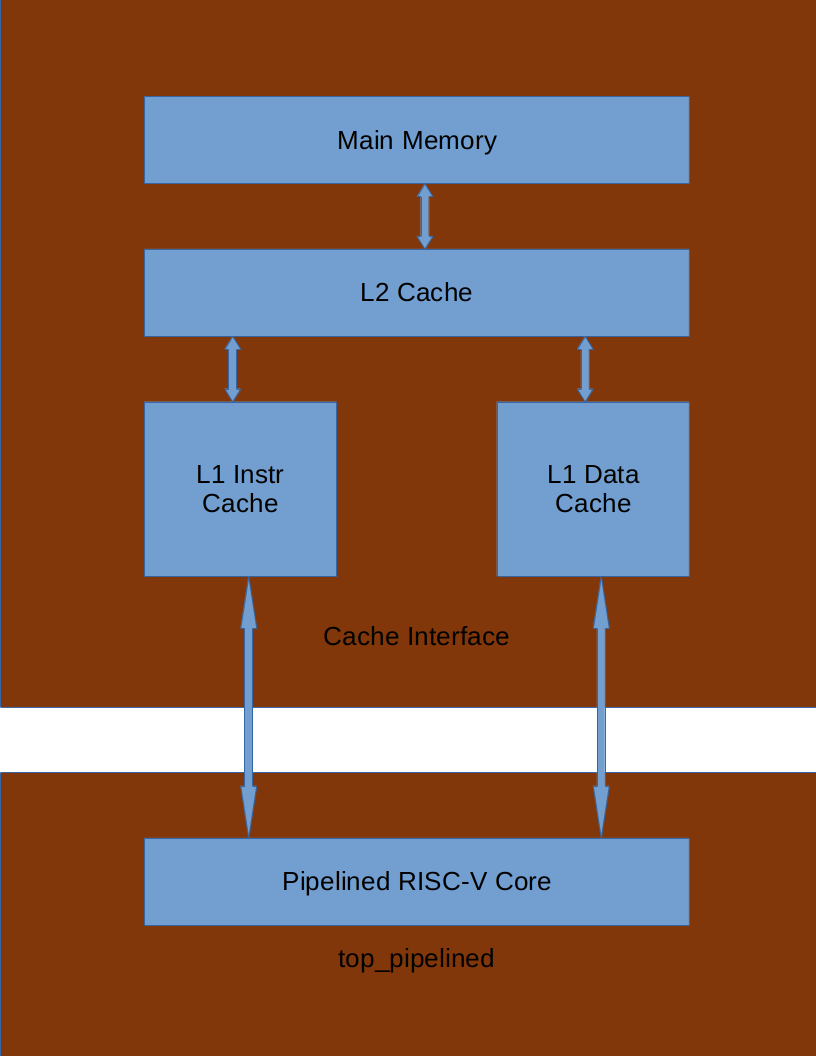
\includegraphics[width=8cm]{cacheproc.png}

Next, we replaced all main memory requests in the processor to use this interface. Then, we made our system have a multi layer cache (L1 and L2). To do this, we used the lab5 code as is for the 2nd layer. L2 was connected to main memory. We converted the Beveren test to evaluate words to ensure coherency. The single core processor tests all ran at this point.

\subsection{Word to Lines}

To handle loading programs into main memory as lines, we used Martin's script from Piazza (\lstinline|arrange_mem.py|) with a few notable bug fixes.
\begin{enumerate}[(1)]
  \item We pad everything with zeroes to fix some issues with addressing in bluespec when there is only a single 0 on a line. We therefore pad with A's and 0's as appropriate
  \item We fix the handling of explicit memory addresses (starting with @) to handle hex values 
\end{enumerate}

\begin{lstlisting}[language=Python]
def to_string(list_of_words):
  list_of_words.reverse()
  output = "".join(list_of_words)
  if not output:
      output = "0"
  list_of_words.clear()
  return "a"*(128-len(output)) + output + "\n"
.....
    for line in input:
    if '@' in line:
        if current_line:
            output.write(to_string(current_line))
        current_word = 0
        num = line[1:-2]
        output.write("@" + str(num) + "\n")
.....
\end{lstlisting}

\section{Multi-core Processor}

This section covers our implementation of a dual-core processor, its parent protocol processor, and its cache hierarchy.

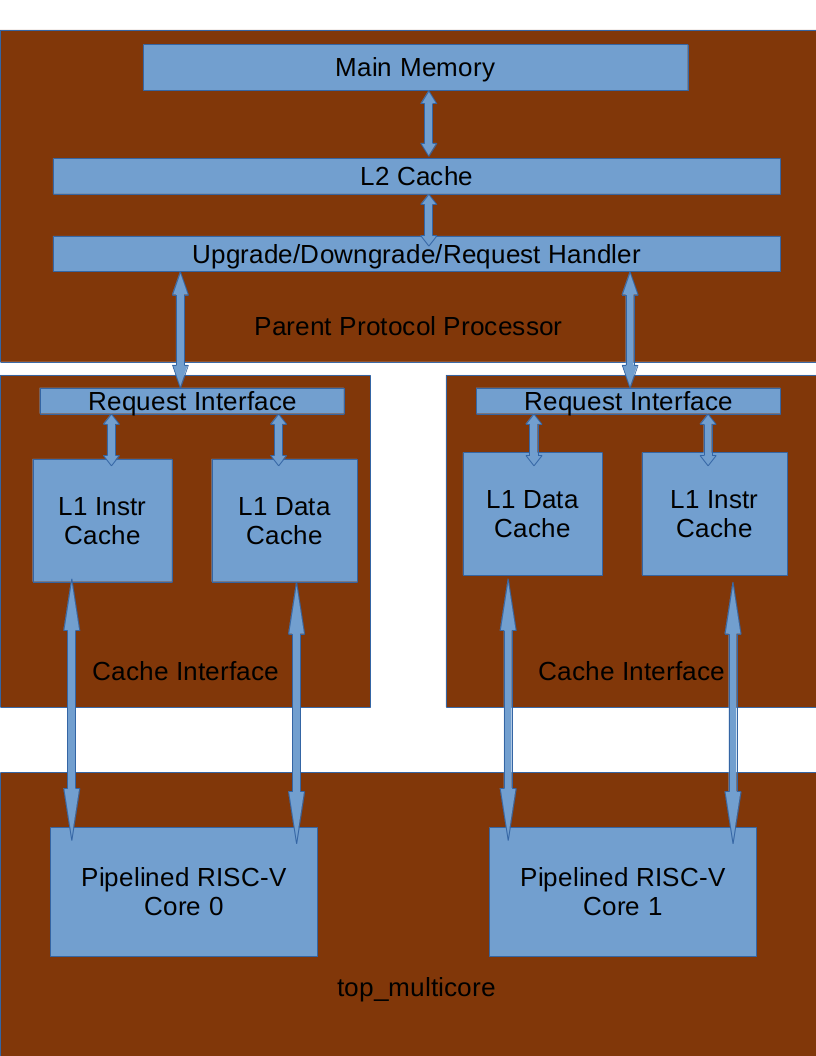
\includegraphics[width=10cm]{multicore.png}

\subsection{Processor Requests}

The processor aspect changed very little. Here, we simply instantiate two cores, but set one core to start at $pc=0$ and the other to start at $pc=4096$. Requests to cache/memory are handled separately for each. This setup allows us to run different code on each core and potentially add more cores.

\subsection{Cache Updates}

We instantiate one cache interface (each has a data and instruction cache) for each core. The Cache Interface now only handles the immediate requests, with higher levels abstracted to the parent protocol processor. Here, we have a new interface as a result.

\begin{lstlisting}
interface CacheInterface;
    method Action sendReqData(CacheReq req);
    method ActionValue#(Word) getRespData();
    method  Action sendReqInstr(CacheReq req);
    method ActionValue#(Word) getRespInstr();
    method ActionValue#(MainMemReq) sendReq();
    method ActionValue#(CacheReq) upgrade();
    method Action downgrade(CacheReq req);
    method Action connectL2L1Cache(MainMemResp resp);
endinterface
\end{lstlisting}

We implement a \lstinline{sendReq} to handle any existing requests to the L2 cache. The \lstinline|upgrade| function forwards any data write requests to the Parent Protocol Processor (PPP). Downgrade receives the upgrades from other caches and processes them. 

Notably, downgrades are handled slightly differently than normal write. Here, we only handle hit logic, because we only care to update old versions of data, not lack thereof. Furthermore, all writes are immediately enqueued to the Parent Protocol Processor to make sure future reads from other cores are getting the latest values.

\subsection{Parent Protocol Processor}

The Parent Protocol Processor is the sole part where the two cores interact with each other. Therefore, all data/cache coherency must be handled by the PPP. Upgrades are immediately forwarded to other caches in the upgrade/downgrade handler. Writes are also enqueued to the L2 cache to ensure the latest data is available to all cores. Any other requests for lower level evictions or loads for instructions and data are sent directly to the L2 cache. 

The PPP takes in an input of the two core's cache interfaces which are both created by the processor. 

\begin{lstlisting}
module mkParentProtocolProcessor#(CacheInterface core1, CacheInterface core2)(ParentProtocolProcessor);
\end{lstlisting}

To handle multiple cores, we identify each core as 0 or 1. Any requests from each of these cores that are sent to L2 cache are tagged in a FIFO queue with a label so that when receiving a response, we return the data to the core in FIFO order.

Note that instruction/data labelling is still handled within the L1 cache to PPP interface. The PPP uses \lstinline{connectL2L1Cache} to return the data from L2 for processing.

% Our first plan is to implement a multi-core processor. To do this, we will build off of our Processor and Cache labs and implement a shared cache hierarchy that maps to a main memory unit.\\ 

% 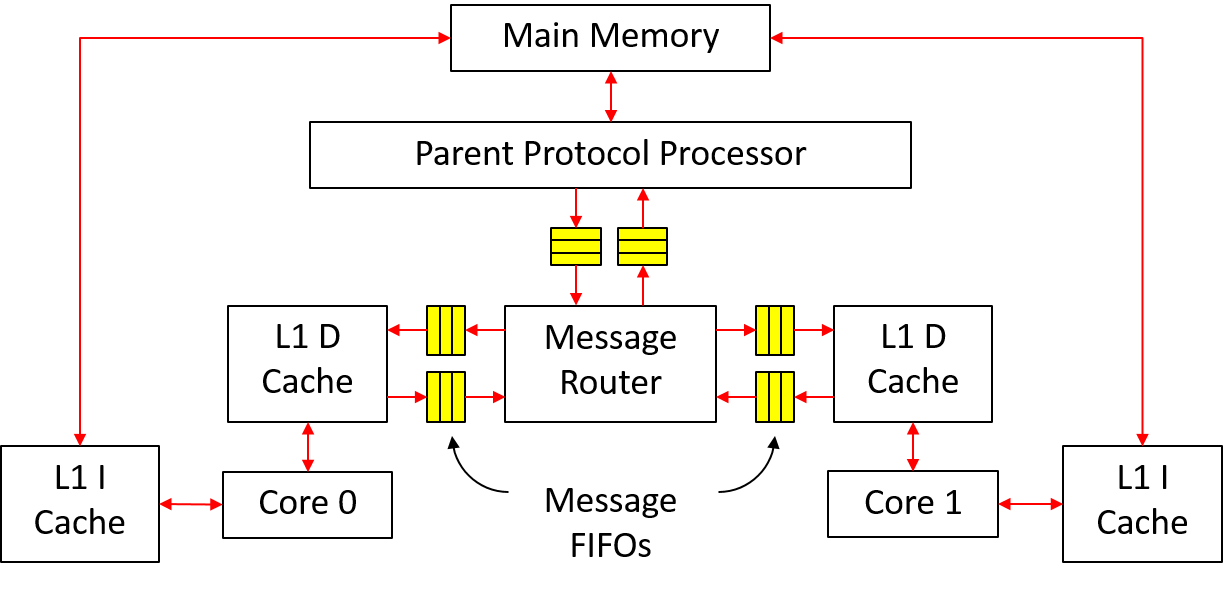
\includegraphics[width=10cm]{system.png}\\

% We will include two cores, so the processor will be able to run two sets of instructions at the same time. 
% We will also include a series of RISC-V cores for each thread/each program. 
% These cores communicate using a message router to enqueue memory requests. Each core shares a single memory for instruction and data accesses so we will work to develop a hierarchy that will allow shared data usage. This means that higher cache levels will have to force an upgrade on the cache when shared core memory is used to avoid overwrites. Each core should be modular and easily scaled to meet the requirements of the system.

% We will have our system consist of a variety of parts. 

% The first is the message FIFO. This is used to transfer upgrade and downgrade responses in a cache hierarchy. This works by having a response FIFO and a request FIFO that together form the message FIFO with associated logic. 

% We then have a message router to connect all the cores' L1 caches to the parent protocol processor. This part will send messages from the parent to the right L1 cache and vice versa. 

% Next, we will have a L1 data cache for each core. This is generally a normal cache interface.

% Finally, we have the parent protocol processor which will handle all the messages to and fro memory and the cache. It handles upgrade and downgrade requests. 

% Multi-core processor and run on FPGA
\section{FPGA}

This section covers our usage of the AWS FPGA server to run our program. Before we could run our code on the server, we had to make some changes to match the appropriate interfaces.

\begin{enumerate}[(1)]
  \item The main memory worked through an AWS interface that expected an ICache and DCache
  \item The RISC-V cores needed a start method
  \item The MMIO was no longer emulated in the processor and was handled by the AWS interface
\end{enumerate}

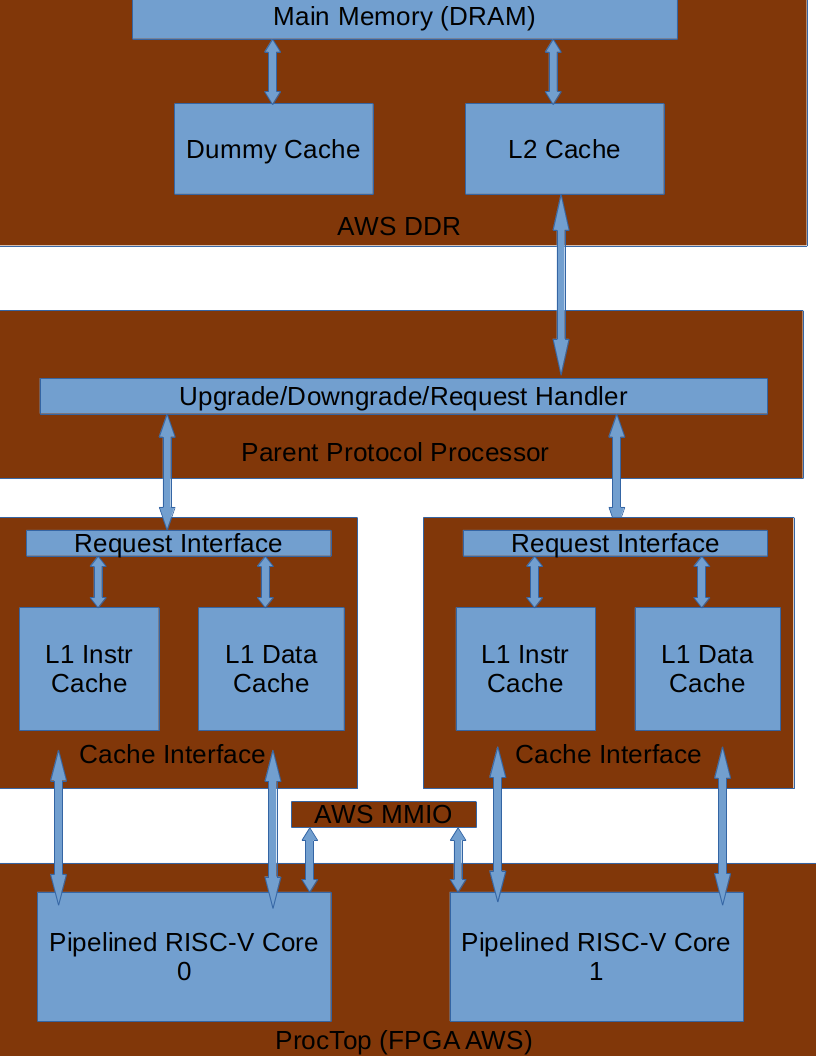
\includegraphics[width=10cm]{fpga.png}

To fix these, we first abstracted the L2 cache out of the ParentProtocolProcessor and let it be part of the AWS DDR interface. We also used a single L2 cache for both cores, instructions and data, so we used only the L2 cache as part of the interface. We made a dummy cache for instructions. Then, we used FIFO ordering again to place MMIO requests and handle responses for each core. Finally, we instantiated both cores and their appropriate caches in the main file to run the programs.

\begin{lstlisting}
let mmioIfc = (interface MMIOInput;
  interface ind = ind;
  method Bit#(32) getTick = tick._read;
endinterface);

let mmioHandler <- mkMMIOHandler(mmioIfc);

Cache cacheL2 <- mkDCache;
Cache cacheL2dummy <- mkDCache;

let memInput = (interface MemInput;
  interface ind = ind;
  method getTick = tick._read;
  interface dCache = cacheL2;
  interface iCache = cacheL2dummy;
  endinterface);
let memController <- mkMemController(memInput);

CacheInterface cache1 <- mkCacheInterface(0);
CacheInterface cache2 <- mkCacheInterface(1);
ParentProtocolProcessor ppp <- mkParentProtocolProcessor(cache1, cache2, ind, cacheL2);

RVIfc rv_core1 <- mkpipelined(0,0);
RVIfc rv_core2 <- mkpipelined(4096,1);
\end{lstlisting}

This initialization allows us to run our code in the AWS system. We successfully compiled our code on the server. However, we were not able to get it fully running in time, due to some memory addressing issues. We are in the process of debugging this with Miguel at the time of writing. 
% Furthermore we plan to run this system on an FPGA unit. This unit will be cloud based and provided by the 6.175 instructors. Since the multi-core processor will likely only run on the server-based unit rather than the small FPGA, we will use the server-based one. We expect that this will involve some work with Verilog and learning to program the controllers. The Bluespec compiler will generate the Verilog code, from which we will use the associated synthesizing tools to push to the FPGA. 

% \section{Other}

% We expect that we will have to first merge our code from the Processor and Cache labs to create a fully functioning pipelined processor. We will also add register and memory access bypassing. We will also have to modify these afterward to implement the aforementioned properties. This will still be implemented in a four stage pipelined processor.

\section{Tests \& Evaluation}

The testing of our code is broken up into modules, basic tests, and then our exhaustive evaluation.

\subsection{Cache Evaluation}
To test the cache, we modified Beveren to handle words and to run on two levels of caches. We made a nested cache as follows:
\begin{lstlisting}
rule connectCacheL1L2;
  let lineReq <- cache.getToMem();
  cache2.putFromProc(lineReq);
endrule
rule connectL2L1Cache;
  let resp <- cache2.getToProc();
  cache.putFromMem(resp);
endrule
rule connectCacheDram;
  let lineReq <- cache2.getToMem();
  mainMem.put(lineReq);
endrule
rule connectDramCache;
  let resp <- mainMem.get;
  cache2.putFromMem(resp);
endrule
\end{lstlisting}
Note that our reference memory was made to load the program data and use Word size data blocks with 32-bit (really 30-bit by RISC-V specs) addressing.
\begin{lstlisting}
// MAIN MEM FAST
BRAM_Configure cfg = defaultValue();
cfg.loadFormat = tagged Hex "mem.vmh";
BRAM1PortBE#(Bit#(30), Word, 4) bram <- mkBRAM1ServerBE(cfg);
DelayLine#(10, Word) dl <- mkDL(); // Delay by 10 cycles

//MAIN MEM
BRAM_Configure cfg = defaultValue();
cfg.loadFormat = tagged Hex "memlines.vmh";
BRAM1Port#(LineAddr, MainMemResp) bram <- mkBRAM1Server(cfg);
DelayLine#(20, MainMemResp) dl <- mkDL(); // Delay by 20 cycles
\end{lstlisting}

\subsection{Simple Processor Tests}

We began our tests by running the same code on both cores (basically the tests from lab4 with a new init.S provided by Thomas).

\begin{lstlisting}[language=RSVAssembler]
.section ".text.init0"
#  .text
  .globl _start
_start:
...
  li  x10,0
...
  li sp, 0xFFFFFF0 // Stack for Processor 0
  call main
  li x10, 0
  call exit
1:
  j 1b

  .align 6
.section ".text.init1"
#  .text
#  .align 6
...
  li  x10,1 // PUT 1, the core ID in register x10
...
  li sp, 0xF000000 // Stack for processor 1
  call main
  li x10, 0
  call exit
1:
  j 1b
\end{lstlisting}

This separates the stacks and calls \lstinline|main(0)| on core0 and \lstinline|main(1)| on core1.

All tests from lab4 ran correctly with this updated system to run the same program on both cores.

\subsection{Basic Multicore Test}

The provided multicore test runs two threads to ensure data access works between the two's writes and reads. In essence, both must pull the latest written data.

\begin{lstlisting}[language=C]
static volatile int input_data[8] = {0,1,2,3,4,5,6,7};
static volatile int flag = 0;
static volatile int acc_thread0 = 0;
void program_thread0(){
  for (int i = 0; i < 4; i++) {
      acc_thread0 += input_data[i];
  }
  char *p;
  while (flag == 0); // Wait until thread1 produced the value
  if (flag + acc_thread0 == 28) {
      for (p = s; p < s + 8; p++) putchar(*p);
  } else {
      for (p = f; p < f + 8; p++) putchar(*p);
  }
}

void program_thread1(){
  int a = 0;
   for (int i = 0; i < 4; i++){
      a += input_data[4+i];
   }
  flag = a;
  while(1);
}
\end{lstlisting}
In this test, we see we have three variables instantiated in shared memory. These are edited by each thread for inter-thread communication. This test makes sure that a write in thread 1 can be read in thread 0 before continuing. This test works successfully.

\subsection{Distributed Matrix Multiply}

Our prime test of evaluation is our matrix multiply distributed across two cores. We started with the single core matrix multiply and split the calculations across two cores. 

This is the original code of interest where the entire 16x16 matrix is calculated sequentially.
\begin{lstlisting}[language=C]
int sum;
for (int i = 0; i < 16; i++)
{
    for (int j = 0; j < 16; j++)
    {
        sum = 0;
        for (int k = 0; k < 16; k++)
        {
            sum += multiply(a[i][k], b[k][j]);
        }
        putchar(sum);
        c[i][j] = sum;
    }
}
if (arrEquals(expected, c))
{
    exit(0);
}
else
{
    exit(1);
}
\end{lstlisting}
We converted this code to calculate the first and second 8 rows simultaneously.
\begin{lstlisting}[language=C]
void program_thread0(){
  int sum;
  for (int i = 0; i < 8; i++)
  {
      for (int j = 0; j < 16; j++)
      {
          sum = 0;
          for (int k = 0; k < 16; k++)
          {
              sum += multiply(a[i][k], b[k][j]);
          }
          c[i][j] = sum;
          putchar(sum);
      }
  }

  while (flag == 0); // Wait until thread1 produced the value
  if (arrEquals(expected, c))
  {
      exit(0);
  }
  else
  {
      exit(1);
  }

}


void program_thread1(){
  int sum;
  for (int i = 8; i < 16; i++)
  {
      for (int j = 0; j < 16; j++)
      {
          sum = 0;
          for (int k = 0; k < 16; k++)
          {
              sum += multiply(a[i][k], b[k][j]);
          }
          c[i][j] = sum;
          putchar(sum);
      }
  }
  // mostly since the C compiler is too smart to do flag = 1 or something
  int l = 0;
  for (int i = 0; i < 4; i++){
      l += i;
  }
  flag = l;
  while(1);
}
\end{lstlisting}

This code has thread0 compute the first 8 then wait for thread1 to finish the last 8 before checking that it is correct. The complicated flag code in thread1 is there since the compiler is smart and removes the unnecessary write when just setting to 1.

We compare the cycles it takes to run this program on the multicore processor to running to the original on the single core + cache processor.


On the multicore processor, it ran in 2min 22s with 2673485 cycles. The single core did the same calculations in 2min 43s with 5466137 cycles. Note that the time difference is not that different due to the simulator running everything sequentially in effect. However, the number of cycles is roughly half, as expected.

This would hold for any distributed program. Furthermore, running multiple, non-conflicting programs, can be done at the same time, which could only be done sequentially before.

% We propose a series of tests to evaluate our system.
% \begin{itemize}
%     \item Run two different programs, such as two different sorts, on each core
%     \item Run two different sets of instructions
%     \item Distributed matrix multiply that will divide operations between each core
% \end{itemize}

% We will use the timing results on this and a standard single core processor to evaluate the improvement in performance. 
\section{Difficulties}
 TO DO

% \section{Weekly Updates \& Difficulties}
% \subsection{Week 0}
% Initial version of the outline above.
% \subsection{Week 1}
% We have outlined above in more detail our plans to implement our system in the coming weeks. Next week we will start on the actual code for the Multi-core processor. Eventually we will start learning about FPGAs.
% \subsection{Week 2}
% Worked to create a L1 and L2 cache within a single core processor. Worked to merge the cache code with the RISC-V processor code. We created a two layer cache with 32-bit addressing.
% \subsection{Week 3}
% We finished merging the cache into the processor. This functions as a shared L2 cache for data and instructions, while each has its own L1 cache. L2 is connected to a single ported main memory which stores lines of data. L1 returns words. L2 is twice the size as L1. The processor uses a new cache interface in lieu of directly connecting to memory. We also started implementing the multicore processor, specifically the aforementioned parent protocol processor. We will adjust the cache hierarchy to match. We will keep a shared L2 cache before main memory. 

% % 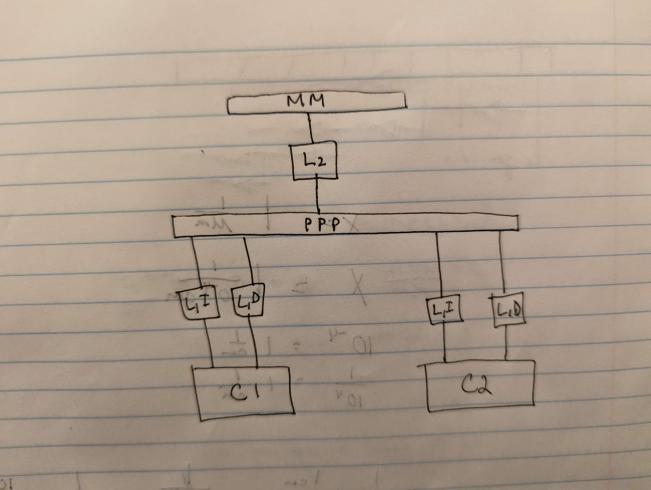
\includegraphics[width=10cm]{ppp.jpg}

% \subsection{Week 4}
% % Bonjour, Thomas. Comment ça va? Nous avons connecté le cache au processeur. Nous avons créé le processeur de protocole parent aussi.
% We incorporated the multicore tests provided and fixed all of our errors in the PPP and cache. We still are having some errors with the multicore test not producing the expected result. We started setup for the FPGA on AWS.

% \subsection{Week 5}

% We finished the multicore processor and PPP. We converted the code to work on the FPGA. However, the FPGA memory reads failed, and we are in the process of debugging it with Miguel. We created a distributed matrix multiply to evaluate our system. 



\section{Sources}

http://csg.csail.mit.edu/6.175/labs/project-part2.html
\\
Course material from Canvas

\end{document}
